% Options for packages loaded elsewhere
\PassOptionsToPackage{unicode}{hyperref}
\PassOptionsToPackage{hyphens}{url}
%
\documentclass[
]{article}
\usepackage{amsmath,amssymb}
\usepackage{lmodern}
\usepackage{iftex}
\ifPDFTeX
  \usepackage[T1]{fontenc}
  \usepackage[utf8]{inputenc}
  \usepackage{textcomp} % provide euro and other symbols
\else % if luatex or xetex
  \usepackage{unicode-math}
  \defaultfontfeatures{Scale=MatchLowercase}
  \defaultfontfeatures[\rmfamily]{Ligatures=TeX,Scale=1}
\fi
% Use upquote if available, for straight quotes in verbatim environments
\IfFileExists{upquote.sty}{\usepackage{upquote}}{}
\IfFileExists{microtype.sty}{% use microtype if available
  \usepackage[]{microtype}
  \UseMicrotypeSet[protrusion]{basicmath} % disable protrusion for tt fonts
}{}
\makeatletter
\@ifundefined{KOMAClassName}{% if non-KOMA class
  \IfFileExists{parskip.sty}{%
    \usepackage{parskip}
  }{% else
    \setlength{\parindent}{0pt}
    \setlength{\parskip}{6pt plus 2pt minus 1pt}}
}{% if KOMA class
  \KOMAoptions{parskip=half}}
\makeatother
\usepackage{xcolor}
\IfFileExists{xurl.sty}{\usepackage{xurl}}{} % add URL line breaks if available
\IfFileExists{bookmark.sty}{\usepackage{bookmark}}{\usepackage{hyperref}}
\hypersetup{
  pdftitle={Exploring the seasonal variation in electric vehicle charging in New Zealand},
  pdfauthor={Pablo Paulsen},
  hidelinks,
  pdfcreator={LaTeX via pandoc}}
\urlstyle{same} % disable monospaced font for URLs
\usepackage[margin=1in]{geometry}
\usepackage{graphicx}
\makeatletter
\def\maxwidth{\ifdim\Gin@nat@width>\linewidth\linewidth\else\Gin@nat@width\fi}
\def\maxheight{\ifdim\Gin@nat@height>\textheight\textheight\else\Gin@nat@height\fi}
\makeatother
% Scale images if necessary, so that they will not overflow the page
% margins by default, and it is still possible to overwrite the defaults
% using explicit options in \includegraphics[width, height, ...]{}
\setkeys{Gin}{width=\maxwidth,height=\maxheight,keepaspectratio}
% Set default figure placement to htbp
\makeatletter
\def\fps@figure{htbp}
\makeatother
\setlength{\emergencystretch}{3em} % prevent overfull lines
\providecommand{\tightlist}{%
  \setlength{\itemsep}{0pt}\setlength{\parskip}{0pt}}
\setcounter{secnumdepth}{-\maxdimen} % remove section numbering
\usepackage{float}
\floatplacement{figure}{H}
\usepackage{comment}
\ifLuaTeX
  \usepackage{selnolig}  % disable illegal ligatures
\fi

\title{Exploring the seasonal variation in electric vehicle charging in
New Zealand}
\author{Pablo Paulsen}
\date{18/02/2022}

\begin{document}
\maketitle

\begin{equation}
\label{eq1}
E_{m,R} = \eta_{m,R} \times d_{m,R}
\end{equation}

\ref{eq1}

\hypertarget{data-exploration}{%
\subsection{Data Exploration}\label{data-exploration}}

\hypertarget{flip-the-fleet-data-exploration}{%
\subsubsection{Flip the Fleet Data
Exploration}\label{flip-the-fleet-data-exploration}}

Distance traveled and vehicle energy efficiency (km/kWh) by month, as
well as the region of the vehicle was collected from the on-board
computers of 1259 electric vehicles (EV) between 2017 and 2021 by Flip
the Fleet \cite{ftf}.

Energy economy (Wh/km) was calculated as the inverse of efficiency
(km/kWh). Energy economy will be used instead of efficiency in the
modelling in this work for reasons that will become apparent later in
the analysis.

A monthly weighted average energy economy was calculated for the whole
of New Zealand and then for each region. The monthly averages were
weighted using the distance traveled to give more weighting to vehicles
with higher km traveled in that month. This was done using the formula

\[\bar{x} = \frac{\sum_{i}^{n} (d_i\times x_i)}{\left(\sum_{i}^{n} d_i\right)\times n}\]

\begin{figure}
\centering
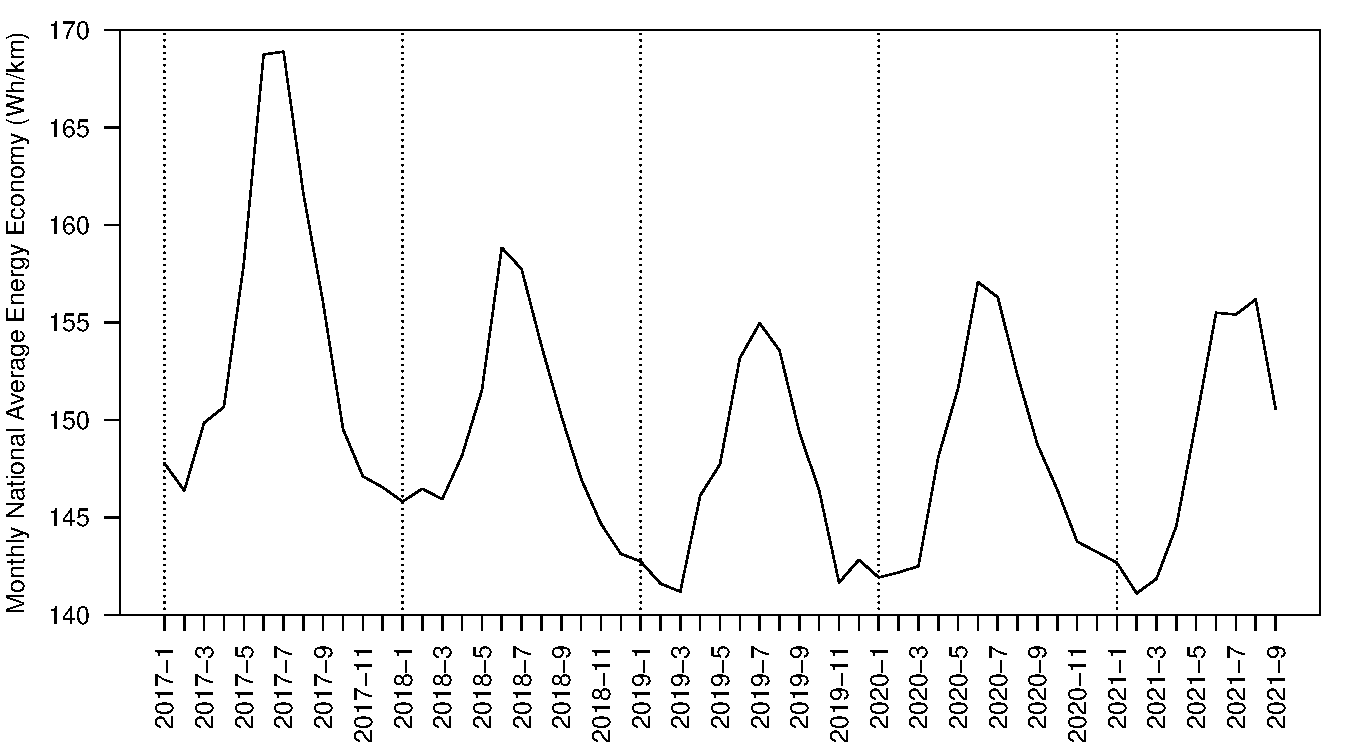
\includegraphics{mixed_model_files/figure-latex/consum_plot-1.pdf}
\caption{National monthly average energy economy of Flip the Fleet
vehicles\label{fig:consum_plot}}
\end{figure}

Figure \ref{fig:consum_plot} shows there is a clear seasonal trend in
the national monthly average energy economy of Flip the Fleets vehicles.

A time series decomposition is used to isolate the seasonal trend in
energy economy from the overall trend. This can be done for all regions
of NZ combined and also for each region individually.

\begin{figure}
\centering
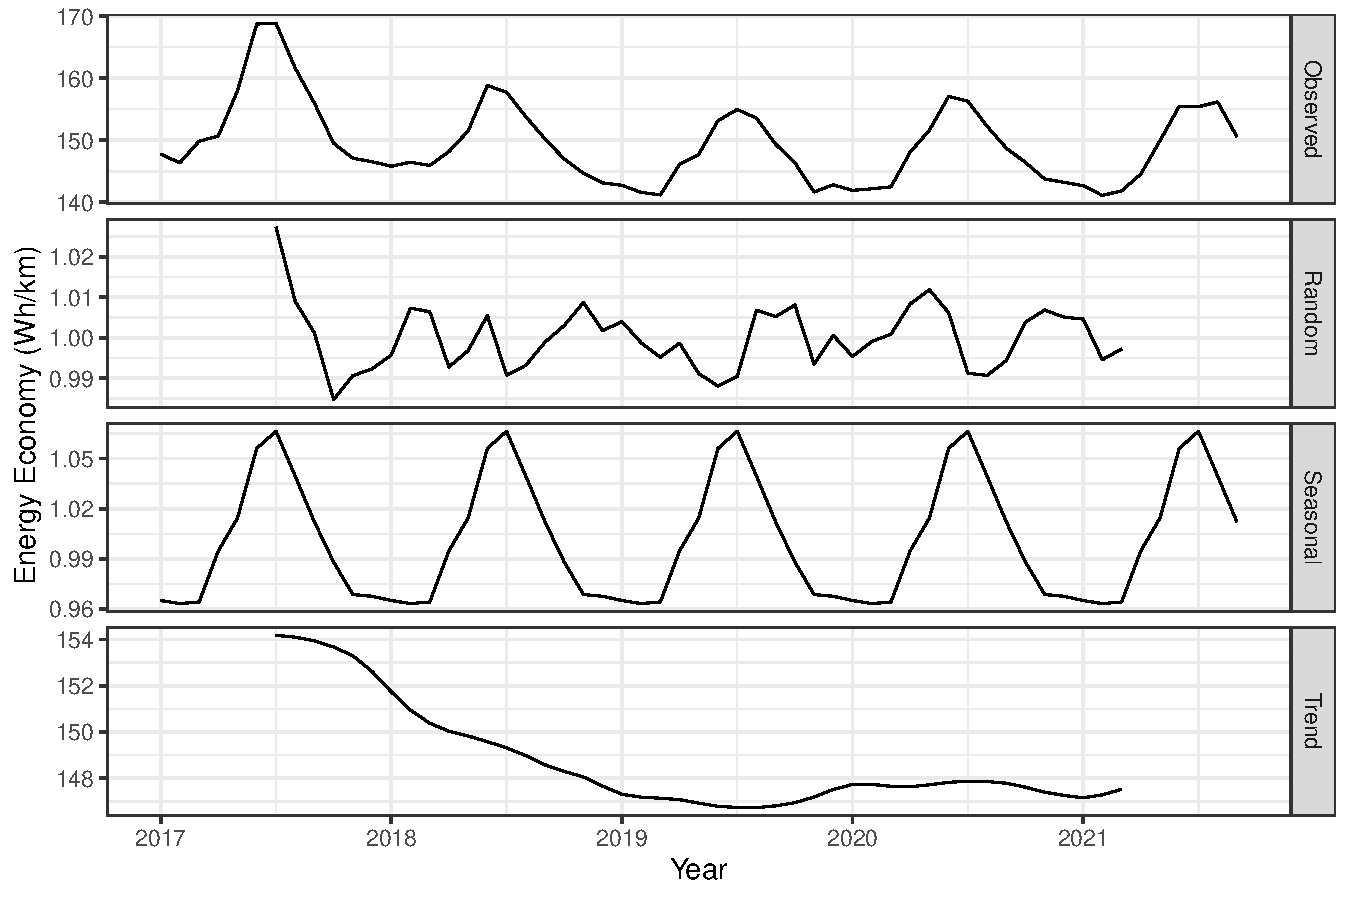
\includegraphics{mixed_model_files/figure-latex/consum_decomp_plot-1.pdf}
\caption{Multiplicative time series decomposition of Flip the Fleet
average energy economy for all of NZ\label{fig:consum_decomp_plot}}
\end{figure}

\begin{figure}
\centering
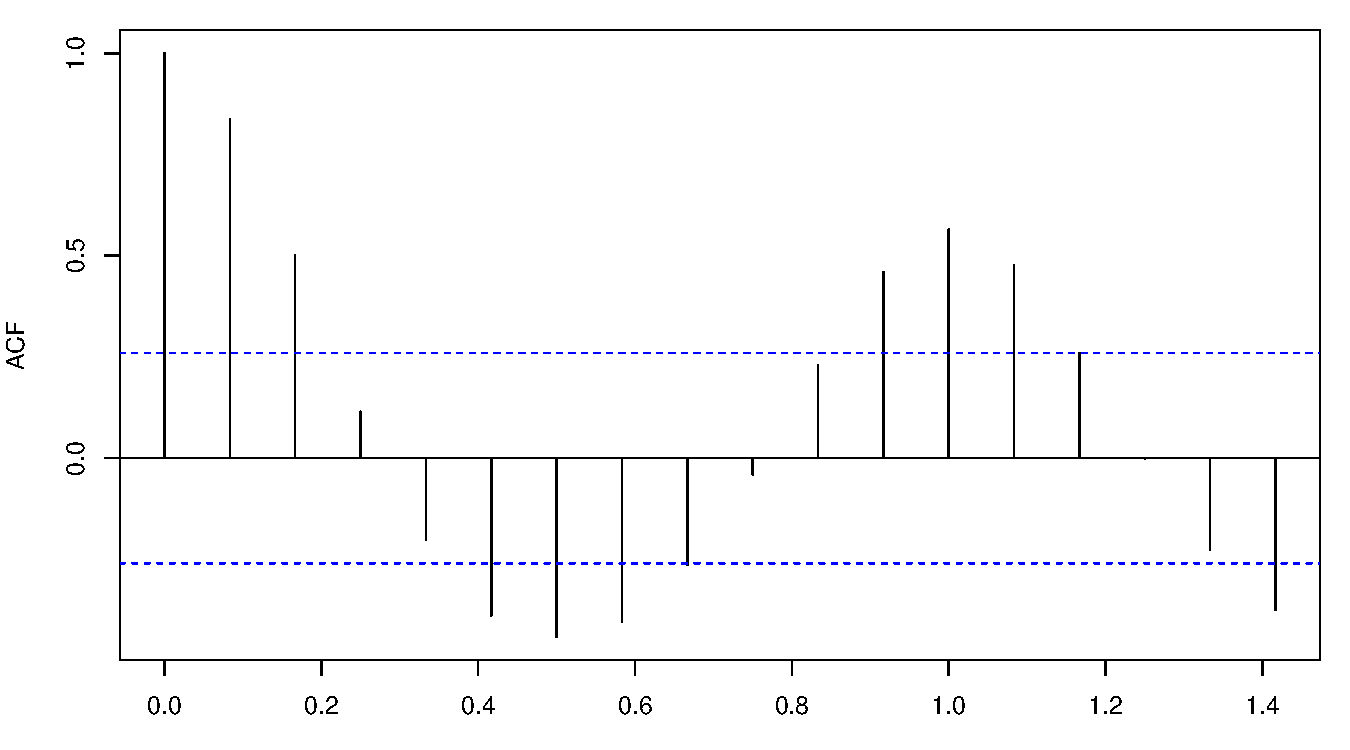
\includegraphics{mixed_model_files/figure-latex/acf_consum-1.pdf}
\caption{Autocorrelation plot of Flip the Fleet average energy economy
for all of NZ\label{fig:acf_consum}}
\end{figure}

The time series decomposition (Figure \ref{fig:consum_decomp_plot})
shows a very clear seasonal trend. The autocorrelation plot (Figure
\ref{fig:acf_consum}) shows that this yearly trend is significant. This
seasonal trend goes from 0.96 times the mean energy economy in February
to 1.07 times the mean energy economy in July, a peak to peak difference
of 10.7\%.

Past research shows that a majority of the seasonal variation in EV
efficiency is due to cabin temperature control\cite{ev_range}. This
would suggest that EV energy economy is correlated with heating degree
days. To test this hypothesis, as NZ weather differs significantly by
region, we must limit the comparison to a single region and compare it
to that regions weather at the same period of time.

In order to do this, hourly weather data from 2017 to 2021 was collected
from the NIWA National Climate Database for 14 regions around New
Zealand that best correspond to the regions of the Flip the Fleet
vehicles. Using the regional hourly temperatures, monthly heating degree
days (HDD) and cooling degree days (CDD) were imputed using base
temperatures of 16\(^\circ\)C and 22\(^\circ\)C respectively. These base
temperatures were selected to represent the range of comfortable
temperatures for most people. Monthly average temperature were also
calculated.

The HDD and CDD was then divided by the length of the month to determine
to average heating/cooling degrees days per day for the month. This is
so that when comparing to other statistics, such as efficiency that are
averaged out rather than summed, there is less bias.

The calculated monthly weather statistics by region was then compared to
the monthly EV data based on the regions of vehicle. This assumes that
most vehicles stay in their own region for a majority of the time.

\begin{figure}
\centering
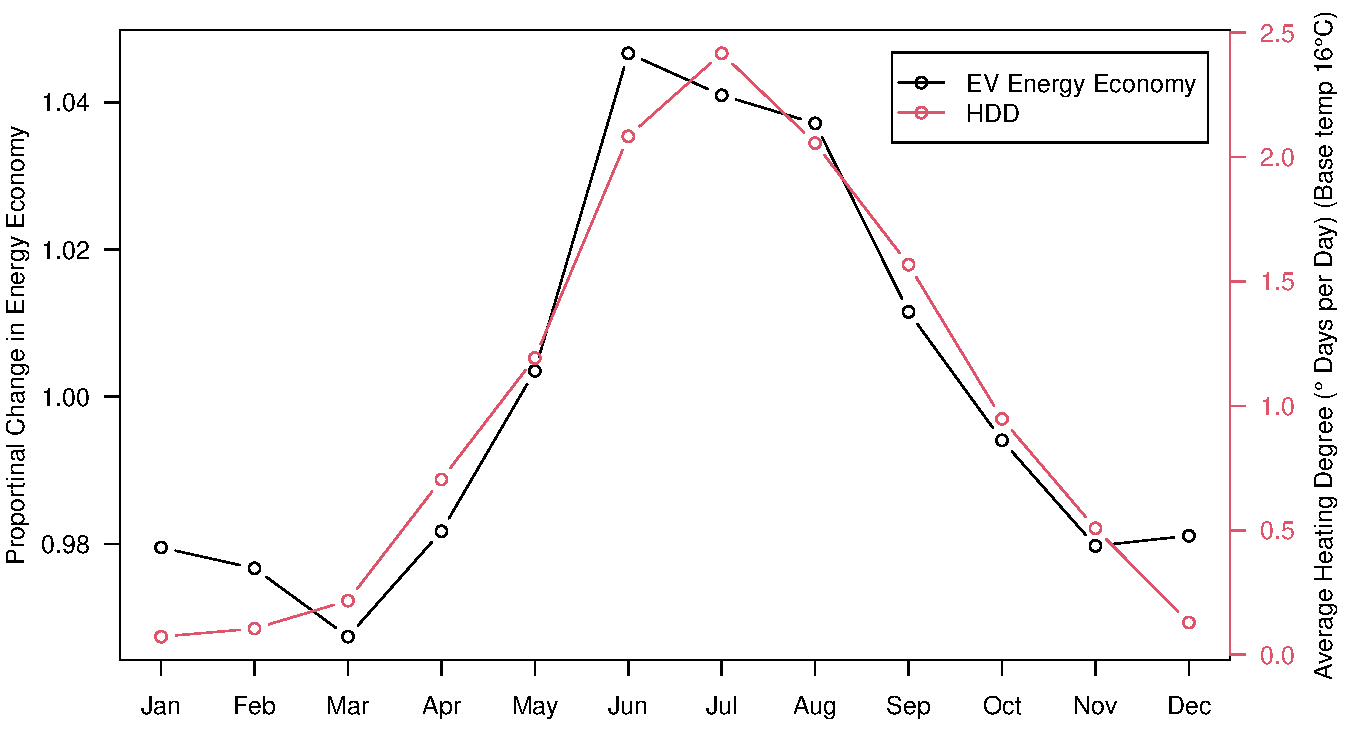
\includegraphics{mixed_model_files/figure-latex/consum_HDD_plot-1.pdf}
\caption{Auckland seasonal HDD and EV energy economy
decompostions\label{fig:consum_HDD_plot}}
\end{figure}

Auckland is used as an example to compare correlation between HDD and
energy economy as it has the largest amount of data and is of most
interest to Vector. Within Auckland, Figure \ref{fig:consum_HDD_plot}
shows very clearly that HDD and energy economy of EVs are highly
correlated. There is a slight increase in energy economy in January and
February and it can be questioned if that is due to AC usage which would
decrease range \cite{ev_range} or other factors such as holiday travel,
often involving highway driving which EVs are generally less efficient
at \cite{ev_highway}. This effect is not obvious in the overall trend
for NZ, so due to the fact that Auckland for the most part is a warmer
climate than the rest of NZ.

\begin{figure}
\centering
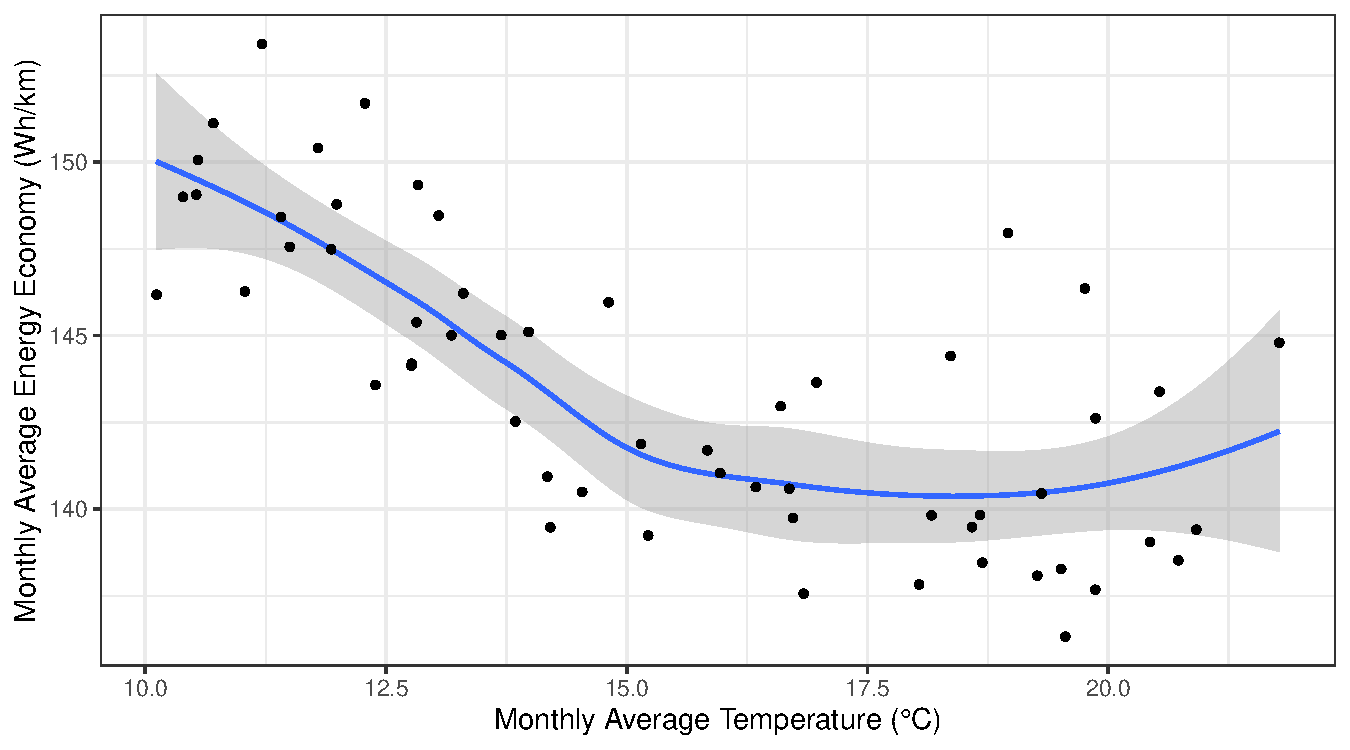
\includegraphics{mixed_model_files/figure-latex/temp_consum_plot-1.pdf}
\caption{Auckland monthly average energy economy by avg
temperature\label{fig:temp_consum_plot}}
\end{figure}

Further exploring the relation between energy economy and weather in
Auckland, Figure \ref{fig:temp_consum_plot} shows a decreasing energy
economy up to around a monthly average temperature of 17.5°C. However,
increasing monthly average temperature past this, there appears to be a
trend towards increasing EV energy economy. As stated previously,
research \cite{ev_range} suggested AC also increases energy economy of
EVs. This suggests it may be worth including both cooling degree days
and heating degree days in the analysis. This could also be useful to
explain the points well above the trend line that may be from a month
where there was both cold and warm days contributing to a high usage of
cabin temperature control, increasing energy economy, but average
temperature would not be able to show this.

\hypertarget{nz-vkt-data-exploration}{%
\subsubsection{NZ VKT Data Exploration}\label{nz-vkt-data-exploration}}

To determine the season impacts of EV charging on our electricity grid
we also need to explore seasonality in driving patterns. A number of
data sets were considered including fuel usage and vehicle kilometers
traveled (VKT) data.

To explore the seasonal trend in fuel usage in NZ, fuel trade data
\cite{fuel_trade} from the Ministry of Business, Innovation and
Employment (MBIE) is used. This data set includes quarterly fuel usage
data broken down by fuel type and sector. This allows the isolation of
petrol usage in domestic land transport, which should provide an
estimate of the fuel usage by light passenger vehicles. Fuel trade data
from 2020 was excluded as lockdowns were not an accurate representation
of the general driving patterns of the NZ population.

\begin{figure}
\centering
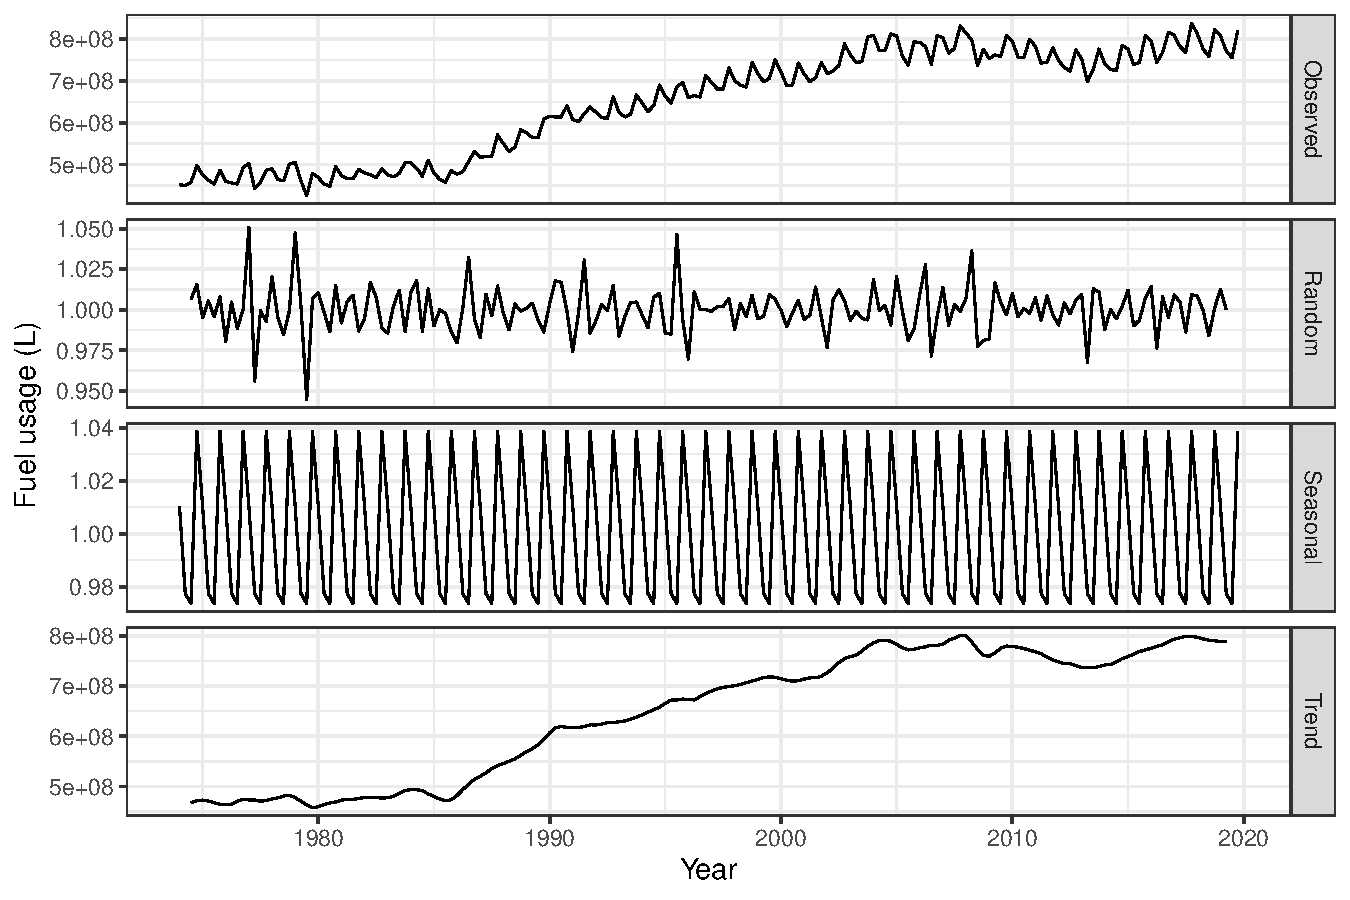
\includegraphics{mixed_model_files/figure-latex/petrol_ts-1.pdf}
\caption{Multiplicative time series decomposition of petrol usage in
domestic land transport\label{fig:petrol_ts}}
\end{figure}

Figure \ref{fig:petrol_ts} time series decomposition shows a seasonal
trend in petrol usage, however, it is of relatively small magnitude
compared to the random variations suggesting this trend may not be
significant.

\begin{figure}
\centering
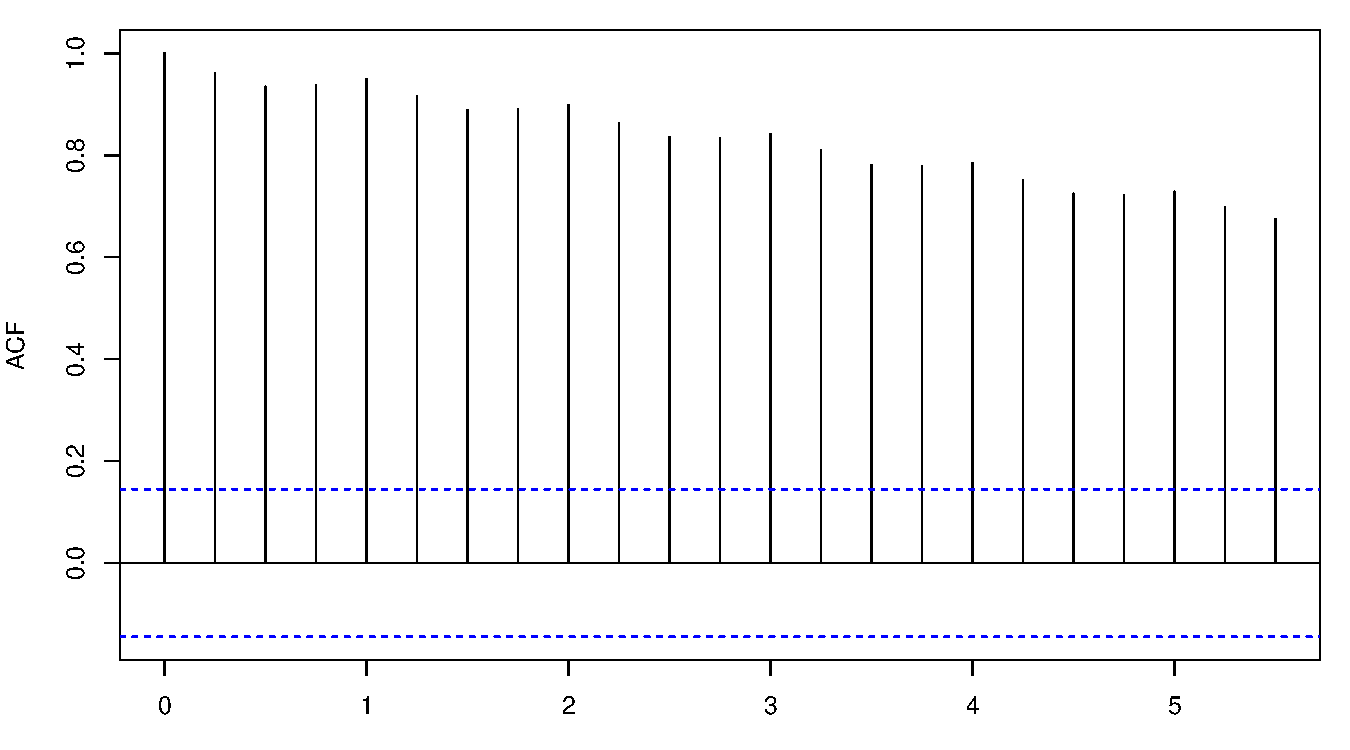
\includegraphics{mixed_model_files/figure-latex/acf_petrol-1.pdf}
\caption{Autocorrelation of petrol usage in domestic land
transport\label{fig:acf_petrol}}
\end{figure}

The autocorrelation plot (figure \ref{fig:acf_petrol}) suggest that
there might be a slight trend in petrol usage however it does not appear
to be of much significance.

Fuel trade data can be compared to the VKT data from the Ministry of
Transport. VKT data including quarterly data of 10 regions plus one
``other'' region was given by Haobo Wang from the Ministry of Transport
for use in this project. Further yearly data for VKT of the ``other''
regions, the vehicle fuel type and vehicle type was collected from the
publicly available fleet statistics page on Ministry of Transport's
website. The quarterly VKT data was then multiplied by the proportion of
VKT that was attributed to light passenger vehicles in that year.

\begin{figure}
\centering
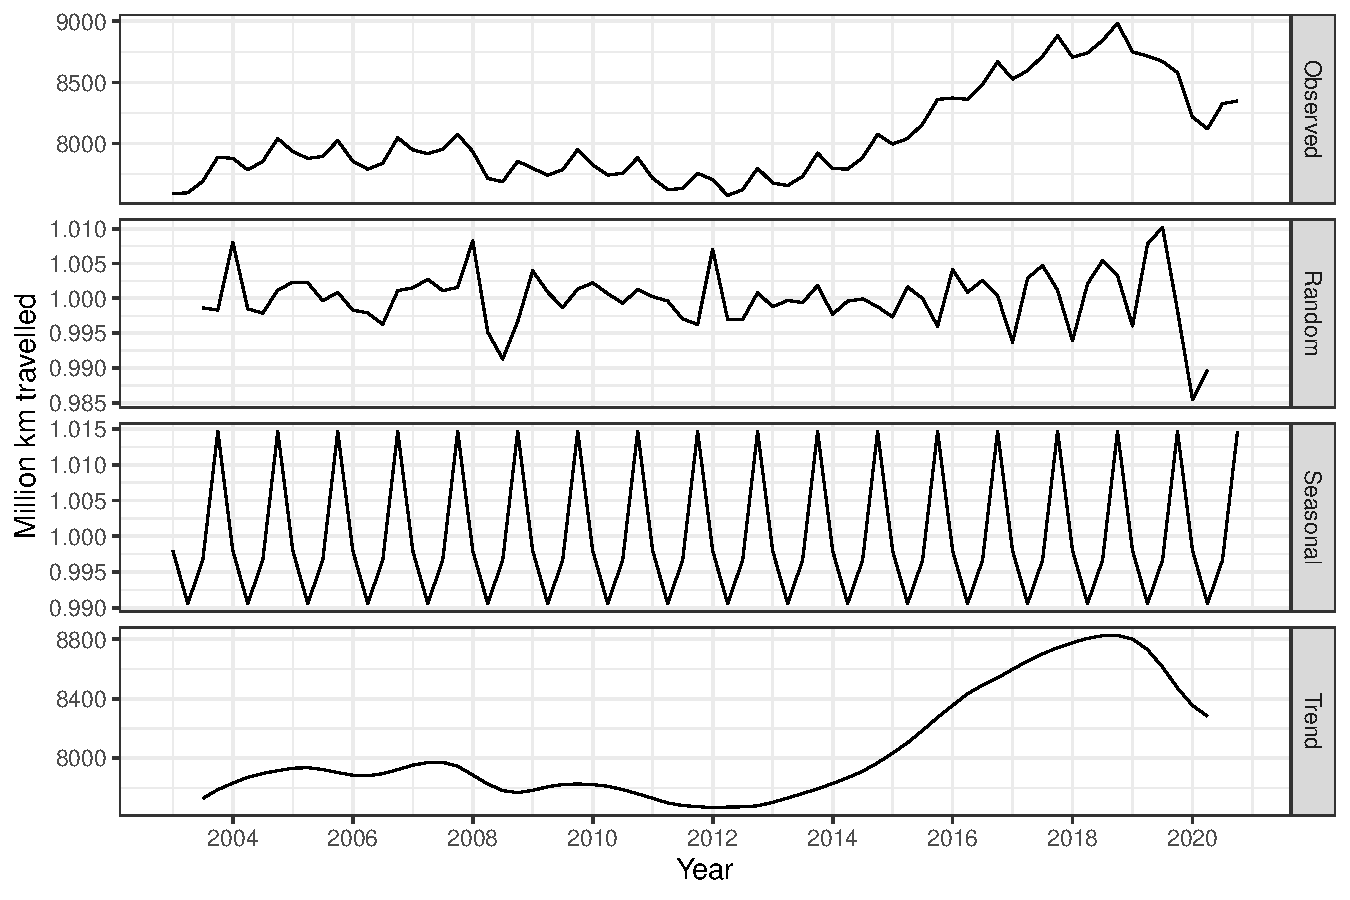
\includegraphics{mixed_model_files/figure-latex/VKT_ts-1.pdf}
\caption{Decomposition of NZ all regions passenger VKT Time
Series\label{fig:VKT_ts}}
\end{figure}

Figure \ref{fig:VKT_ts} shows the time-series decomposition of the NZ
total VKT data shows a clear seasonal trend, albeit smaller than the
trend from the fuel sales data. There is, however, clearly a large
amount of smoothing going on with this data. This is shown in a couple
of different ways including:

\begin{itemize}
\item The drop of VKT due to lockdown which started in 2020 March is already visible in the data from early 2019. 
\item Related to the previous point, the Random component of Time Series Decomposition shows only a 10\% decrease in VKT spread out over a 1 year period from lockdown, compared to 30\% drop in fuel usage during only 1 quarter shown in the MIBE fuel trade data. 
\item Random variation in MIBE fuel trade data shows around a 3 times greater random variation. There could be a seasonal effect on fuel efficiency which could change the seasonal fuel trend relative to VKT, but there is no reason there would be any significant randomness in fuel efficiency so randomness should be of similar magnitude.
\end{itemize}

This smoothing likely occurs due to the method of VKT data collection
using the odometer readings during WoF/CoF. For a majority of vehicles
WoF is only done once a year and in the case of new cars that could be
up to 3 years. This likely causes the data to show less seasonal trend
than may exist in the real world.

Looking at the long term trend, VKT remained largely flat between 2004
and 2012 after which there was a steady but significant increase until
2019. After this, there is a decrease in VKT due to lockdown, which in
this data set for the above reasons likely started showing its effects
in 2019.

\begin{figure}
\centering
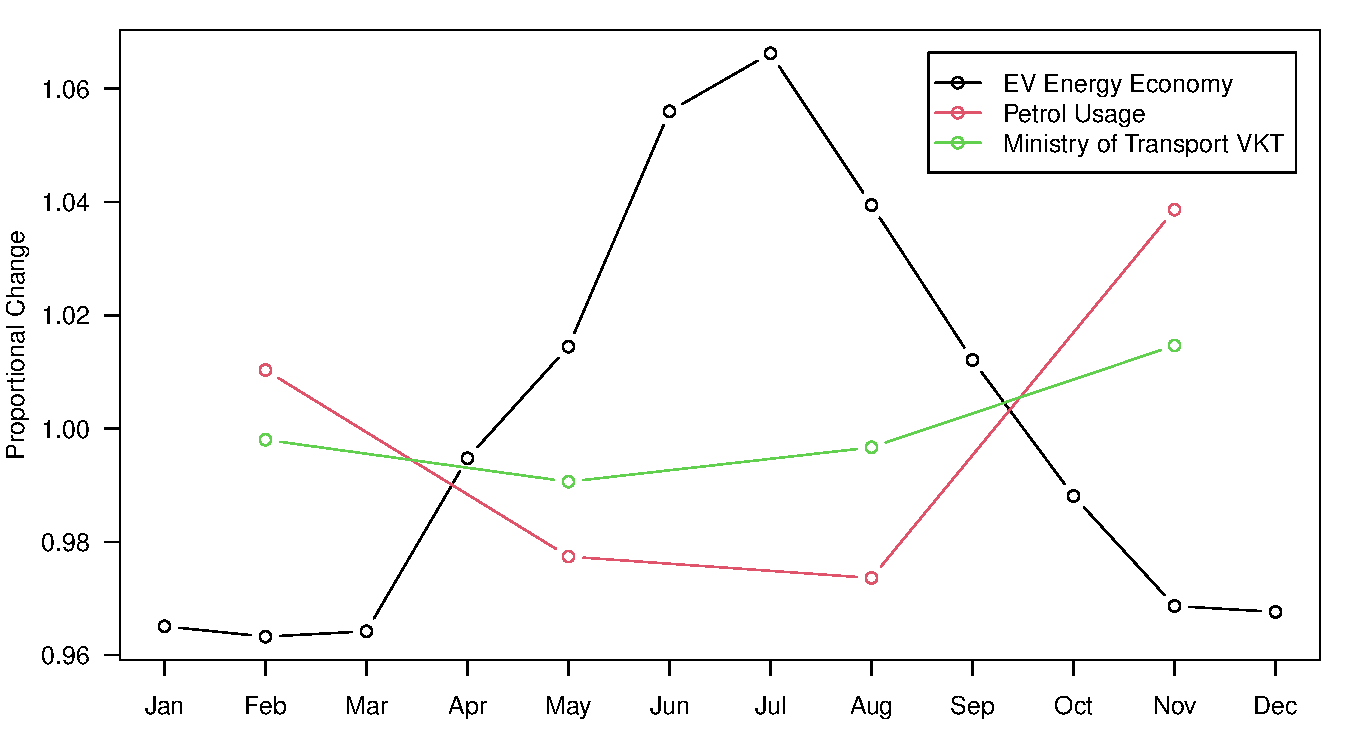
\includegraphics{mixed_model_files/figure-latex/petrol_VKT_vs_eff-1.pdf}
\caption{NZ Seasonal Component Decompostions}
\end{figure}

Looking at the Seasonal trend of Petrol Usage and VKT data from Ministry
of Transport, we can see an obvious decrease in the winter months with a
peak in the 4th quarter likely corresponding to holiday travel. Petrol
Usage shows this variation to be much larger in the VKT data from
Ministry of Transport. It is unclear whether this would be due to the
smoothing effect as was previously discussed regarding the Ministry of
Transport data, or perhaps a change in efficiency for petrol vehicle by
seasons similar to that of the EV. Combining these 2 data sets it is
reasonable to suggest that in New Zealand, compared to the winter (Q2
and Q3) VKT, the true VKT in the summer (Q1 and Q4) is between 1.3\%
higher, as suggested by the VKT data from Ministry of Transport, to 5\%
higher, according to the petrol usage data.

Looking at the seasonal trend of EV energy economy we can see a much
larger increase in energy economy in the winter months, with average
energy economy in July being 10.7\% higher energy economy than in
February. From the plot we can see that when energy economy of EVs
increases, VKT goes down, suggesting that some increase in total power
usage due to EVs increase in energy economy will be countered by a
decrease in VKT. However, the increase in energy economy is much larger
than the decrease in VKT. This, combined with the fact that winter is
when our electricity grid in New Zealand is already under strain due to
heating demand, suggests that if we ignore the relatively small change
in VKT in our model we can effectively model a worst case scenario. Thus
we propose that monthly distance (\(d_{R}\)) in our model is constant
and determined by the yearly regional VKT data from 2019.

\begin{verbatim}
## Linear mixed-effects model fit by REML
##   Data: EV_data 
##        AIC      BIC   logLik
##   170214.8 170495.6 -85072.4
## 
## Random effects:
##  Formula: ~1 | vehicle
##         (Intercept) Residual
## StdDev:     14.0654 9.567276
## 
## Fixed effects:  consumption ~ HDD + CDD + weather_region + model 
##                                         Value Std.Error    DF   t-value p-value
## (Intercept)                         131.26922  0.888502 21322 147.74214  0.0000
## HDD                                   2.48966  0.033265 21322  74.84360  0.0000
## CDD                                   3.57136  0.380127 21322   9.39520  0.0000
## weather_regionUpper Hutt              0.35901  1.198578  1237   0.29953  0.7646
## weather_regionChristchurch           -0.88088  1.210592 21322  -0.72764  0.4668
## weather_regionDunedin                12.96393  1.464586  1237   8.85161  0.0000
## weather_regionHamilton                6.40007  1.889778 21322   3.38668  0.0007
## weather_regionNelson                 -0.91074  2.101970 21322  -0.43328  0.6648
## weather_regionRotorua                 3.39476  1.986034 21322   1.70932  0.0874
## weather_regionClyde                   2.54261  2.798074  1237   0.90870  0.3637
## weather_regionPalmerston North       12.70238  2.444476 21322   5.19636  0.0000
## weather_regionStratford               2.05463  3.545867  1237   0.57944  0.5624
## weather_regionNapier                  5.58418  3.586003  1237   1.55721  0.1197
## weather_regionInvercargill           13.14736  5.208424  1237   2.52425  0.0117
## modelNissan Leaf (30 kWh)             2.42191  1.021163 21322   2.37172  0.0177
## modelNissan Leaf (24 kWh) 2011-2012  12.33770  1.127974 21322  10.93794  0.0000
## modelNissan Leaf (40 kWh)             9.69363  1.832128 21322   5.29091  0.0000
## modelNissan e-NV200 (24 kWh)         28.18869  1.808797 21322  15.58421  0.0000
## modelHyundai Ioniq (EV)             -16.46100  3.034990  1237  -5.42374  0.0000
## modelBMW i3                          -2.02706  3.149512  1237  -0.64361  0.5199
## modelHyundai Kona (EV)                1.01439  3.919889  1237   0.25878  0.7958
## modelRenault Zoe                     11.46407  3.941651  1237   2.90844  0.0037
## modelTesla Model 3                   11.07660  3.986575  1237   2.77847  0.0055
## modelNissan Leaf (62 kWh)            23.01582  4.358462  1237   5.28072  0.0000
## modelKia Niro (EV)                    8.84581  4.923701  1237   1.79658  0.0726
## modelTesla Model S                   63.09123  6.629155  1237   9.51724  0.0000
## modelVolkswagen e-Golf                0.13605  6.612170  1237   0.02058  0.9836
## modelTesla Model-X                   97.73025  7.253438  1237  13.47365  0.0000
## modelKia Soul                         9.14292  8.281533  1237   1.10401  0.2698
## modelMG ZS EV                        24.36115  8.876300  1237   2.74452  0.0061
## modelRenault Kangoo (van)            56.72294  8.428856  1237   6.72961  0.0000
## modelJaguar I-PACE                   92.35962 10.234673  1237   9.02419  0.0000
## modelPeugeot e-208                    8.22841 14.739567  1237   0.55825  0.5768
##  Correlation: 
##                                     (Intr) HDD    CDD    wth_UH wthr_rgnCh
## HDD                                 -0.118                                
## CDD                                 -0.107  0.595                         
## weather_regionUpper Hutt            -0.542 -0.041 -0.013                  
## weather_regionChristchurch          -0.516 -0.067 -0.045  0.393           
## weather_regionDunedin               -0.452 -0.041 -0.008  0.327  0.324    
## weather_regionHamilton              -0.303 -0.022 -0.017  0.249  0.247    
## weather_regionNelson                -0.308 -0.021 -0.008  0.226  0.234    
## weather_regionRotorua               -0.309 -0.027 -0.015  0.237  0.325    
## weather_regionClyde                 -0.207 -0.060 -0.046  0.173  0.170    
## weather_regionPalmerston North      -0.242 -0.011  0.000  0.193  0.192    
## weather_regionStratford             -0.192 -0.016 -0.002  0.139  0.131    
## weather_regionNapier                -0.170 -0.010 -0.012  0.131  0.129    
## weather_regionInvercargill          -0.098 -0.017 -0.005  0.096  0.090    
## modelNissan Leaf (30 kWh)           -0.423 -0.005  0.000  0.040  0.033    
## modelNissan Leaf (24 kWh) 2011-2012 -0.347 -0.005 -0.003  0.002 -0.024    
## modelNissan Leaf (40 kWh)           -0.202 -0.004  0.003 -0.020 -0.037    
## modelNissan e-NV200 (24 kWh)        -0.210 -0.002 -0.001  0.008  0.013    
## modelHyundai Ioniq (EV)             -0.134  0.000  0.000  0.012  0.002    
## modelBMW i3                         -0.130 -0.003  0.002  0.022  0.008    
## modelHyundai Kona (EV)              -0.129 -0.002 -0.001  0.027  0.008    
## modelRenault Zoe                    -0.105 -0.001 -0.004  0.023 -0.059    
## modelTesla Model 3                  -0.095  0.002  0.001 -0.041  0.010    
## modelNissan Leaf (62 kWh)           -0.076 -0.005  0.002 -0.037 -0.018    
## modelKia Niro (EV)                  -0.080  0.003  0.003  0.024 -0.005    
## modelTesla Model S                  -0.096 -0.001  0.001  0.046  0.019    
## modelVolkswagen e-Golf              -0.032 -0.001  0.000 -0.044 -0.023    
## modelTesla Model-X                  -0.098 -0.002 -0.001  0.050  0.041    
## modelKia Soul                       -0.078  0.000  0.000  0.039  0.038    
## modelMG ZS EV                       -0.056 -0.004  0.001  0.022 -0.002    
## modelRenault Kangoo (van)           -0.030  0.000  0.001  0.002 -0.021    
## modelJaguar I-PACE                  -0.056 -0.001  0.001  0.025 -0.011    
## modelPeugeot e-208                  -0.016 -0.004  0.000  0.001 -0.050    
##                                     wthr_D wthr_H wthr_rgnNl wthr_R wthr_rgnCl
## HDD                                                                           
## CDD                                                                           
## weather_regionUpper Hutt                                                      
## weather_regionChristchurch                                                    
## weather_regionDunedin                                                         
## weather_regionHamilton               0.200                                    
## weather_regionNelson                 0.184  0.142                             
## weather_regionRotorua                0.195  0.148  0.138                      
## weather_regionClyde                  0.138  0.106  0.103      0.116           
## weather_regionPalmerston North       0.156  0.377  0.113      0.117  0.082    
## weather_regionStratford              0.108  0.077  0.074      0.077  0.053    
## weather_regionNapier                 0.108  0.084  0.076      0.085  0.060    
## weather_regionInvercargill           0.074  0.062  0.050      0.054  0.043    
## modelNissan Leaf (30 kWh)            0.050 -0.002 -0.004      0.016 -0.024    
## modelNissan Leaf (24 kWh) 2011-2012  0.013 -0.055  0.032     -0.013 -0.001    
## modelNissan Leaf (40 kWh)           -0.018 -0.040  0.003     -0.039  0.001    
## modelNissan e-NV200 (24 kWh)         0.009 -0.005  0.013     -0.009  0.025    
## modelHyundai Ioniq (EV)              0.026 -0.128 -0.028      0.016  0.013    
## modelBMW i3                          0.022 -0.042 -0.005     -0.054 -0.062    
## modelHyundai Kona (EV)               0.026 -0.033  0.030      0.023  0.019    
## modelRenault Zoe                    -0.008  0.015  0.019      0.005  0.012    
## modelTesla Model 3                   0.010 -0.052  0.015      0.011 -0.042    
## modelNissan Leaf (62 kWh)            0.018  0.004 -0.027     -0.032 -0.093    
## modelKia Niro (EV)                  -0.003  0.009 -0.017     -0.072 -0.115    
## modelTesla Model S                   0.039 -0.019  0.025      0.022  0.017    
## modelVolkswagen e-Golf               0.003 -0.002  0.001     -0.004 -0.001    
## modelTesla Model-X                   0.042  0.027  0.028     -0.033  0.018    
## modelKia Soul                        0.034  0.022  0.023      0.022  0.016    
## modelMG ZS EV                        0.019 -0.054  0.012      0.008  0.008    
## modelRenault Kangoo (van)            0.002 -0.002  0.000     -0.203 -0.004    
## modelJaguar I-PACE                   0.021  0.013  0.014      0.009  0.009    
## modelPeugeot e-208                   0.001 -0.002  0.000     -0.008  0.000    
##                                     wth_PN wthr_S wthr_rgnNp wthr_I mNL(3k
## HDD                                                                       
## CDD                                                                       
## weather_regionUpper Hutt                                                  
## weather_regionChristchurch                                                
## weather_regionDunedin                                                     
## weather_regionHamilton                                                    
## weather_regionNelson                                                      
## weather_regionRotorua                                                     
## weather_regionClyde                                                       
## weather_regionPalmerston North                                            
## weather_regionStratford              0.060                                
## weather_regionNapier                 0.068  0.043                         
## weather_regionInvercargill           0.045  0.028  0.030                  
## modelNissan Leaf (30 kWh)            0.019  0.030 -0.002     -0.038       
## modelNissan Leaf (24 kWh) 2011-2012 -0.046  0.034  0.015     -0.033  0.327
## modelNissan Leaf (40 kWh)           -0.034  0.001 -0.037     -0.039  0.191
## modelNissan e-NV200 (24 kWh)         0.000  0.003 -0.034      0.007  0.166
## modelHyundai Ioniq (EV)             -0.140  0.018  0.010      0.001  0.117
## modelBMW i3                         -0.063  0.018 -0.086      0.002  0.116
## modelHyundai Kona (EV)               0.003  0.021  0.016      0.006  0.091
## modelRenault Zoe                     0.013  0.015  0.010      0.003  0.087
## modelTesla Model 3                  -0.010  0.012  0.007     -0.092  0.093
## modelNissan Leaf (62 kWh)            0.004  0.009  0.004     -0.001  0.083
## modelKia Niro (EV)                   0.008  0.011  0.005      0.001  0.076
## modelTesla Model S                   0.006  0.017  0.014      0.007  0.056
## modelVolkswagen e-Golf              -0.001 -0.192  0.000     -0.003  0.047
## modelTesla Model-X                   0.021  0.018  0.015      0.008  0.051
## modelKia Soul                        0.018 -0.122  0.012      0.007  0.041
## modelMG ZS EV                       -0.011  0.009  0.006      0.002  0.041
## modelRenault Kangoo (van)           -0.002  0.002 -0.002     -0.002  0.041
## modelJaguar I-PACE                   0.010  0.009  0.008      0.004  0.035
## modelPeugeot e-208                  -0.001  0.001  0.000     -0.001  0.023
##                                     mNL(k2 mNL(4k mNe-(k mHI(EV mBMWi3 mHK(EV
## HDD                                                                          
## CDD                                                                          
## weather_regionUpper Hutt                                                     
## weather_regionChristchurch                                                   
## weather_regionDunedin                                                        
## weather_regionHamilton                                                       
## weather_regionNelson                                                         
## weather_regionRotorua                                                        
## weather_regionClyde                                                          
## weather_regionPalmerston North                                               
## weather_regionStratford                                                      
## weather_regionNapier                                                         
## weather_regionInvercargill                                                   
## modelNissan Leaf (30 kWh)                                                    
## modelNissan Leaf (24 kWh) 2011-2012                                          
## modelNissan Leaf (40 kWh)            0.201                                   
## modelNissan e-NV200 (24 kWh)         0.149  0.099                            
## modelHyundai Ioniq (EV)              0.114  0.072  0.060                     
## modelBMW i3                          0.103  0.071  0.060  0.050              
## modelHyundai Kona (EV)               0.084  0.053  0.046  0.038  0.030       
## modelRenault Zoe                     0.081  0.053  0.045  0.028  0.026  0.026
## modelTesla Model 3                   0.085  0.055  0.044  0.036  0.032  0.026
## modelNissan Leaf (62 kWh)            0.071  0.046  0.039  0.025  0.033  0.019
## modelKia Niro (EV)                   0.063  0.042  0.034  0.021  0.036  0.017
## modelTesla Model S                   0.050  0.031  0.028  0.024  0.019  0.019
## modelVolkswagen e-Golf               0.041  0.030  0.026  0.013  0.012  0.011
## modelTesla Model-X                   0.044  0.028  0.026  0.015  0.020  0.014
## modelKia Soul                        0.032  0.022  0.022  0.012  0.011  0.011
## modelMG ZS EV                        0.040  0.025  0.021  0.023  0.016  0.015
## modelRenault Kangoo (van)            0.040  0.031  0.024  0.010  0.026  0.008
## modelJaguar I-PACE                   0.032  0.020  0.017  0.011  0.011  0.011
## modelPeugeot e-208                   0.023  0.015  0.012  0.008  0.007  0.007
##                                     mdlRnZ mdlTM3 mNL(6k mKN(EV mdlTMS mdVe-G
## HDD                                                                          
## CDD                                                                          
## weather_regionUpper Hutt                                                     
## weather_regionChristchurch                                                   
## weather_regionDunedin                                                        
## weather_regionHamilton                                                       
## weather_regionNelson                                                         
## weather_regionRotorua                                                        
## weather_regionClyde                                                          
## weather_regionPalmerston North                                               
## weather_regionStratford                                                      
## weather_regionNapier                                                         
## weather_regionInvercargill                                                   
## modelNissan Leaf (30 kWh)                                                    
## modelNissan Leaf (24 kWh) 2011-2012                                          
## modelNissan Leaf (40 kWh)                                                    
## modelNissan e-NV200 (24 kWh)                                                 
## modelHyundai Ioniq (EV)                                                      
## modelBMW i3                                                                  
## modelHyundai Kona (EV)                                                       
## modelRenault Zoe                                                             
## modelTesla Model 3                   0.020                                   
## modelNissan Leaf (62 kWh)            0.020  0.026                            
## modelKia Niro (EV)                   0.018  0.020  0.030                     
## modelTesla Model S                   0.016  0.015  0.011  0.010              
## modelVolkswagen e-Golf               0.012  0.013  0.012  0.007  0.005       
## modelTesla Model-X                   0.012  0.011  0.012  0.015  0.010  0.004
## modelKia Soul                        0.009  0.009  0.007  0.007  0.008  0.031
## modelMG ZS EV                        0.012  0.013  0.008  0.007  0.010  0.004
## modelRenault Kangoo (van)            0.010  0.008  0.016  0.025  0.005  0.004
## modelJaguar I-PACE                   0.012  0.008  0.008  0.007  0.007  0.004
## modelPeugeot e-208                   0.011  0.005  0.006  0.005  0.004  0.004
##                                     mdTM-X mdlKSl mMGZSE mdRK() mJI-PA
## HDD                                                                   
## CDD                                                                   
## weather_regionUpper Hutt                                              
## weather_regionChristchurch                                            
## weather_regionDunedin                                                 
## weather_regionHamilton                                                
## weather_regionNelson                                                  
## weather_regionRotorua                                                 
## weather_regionClyde                                                   
## weather_regionPalmerston North                                        
## weather_regionStratford                                               
## weather_regionNapier                                                  
## weather_regionInvercargill                                            
## modelNissan Leaf (30 kWh)                                             
## modelNissan Leaf (24 kWh) 2011-2012                                   
## modelNissan Leaf (40 kWh)                                             
## modelNissan e-NV200 (24 kWh)                                          
## modelHyundai Ioniq (EV)                                               
## modelBMW i3                                                           
## modelHyundai Kona (EV)                                                
## modelRenault Zoe                                                      
## modelTesla Model 3                                                    
## modelNissan Leaf (62 kWh)                                             
## modelKia Niro (EV)                                                    
## modelTesla Model S                                                    
## modelVolkswagen e-Golf                                                
## modelTesla Model-X                                                    
## modelKia Soul                        0.008                            
## modelMG ZS EV                        0.006  0.005                     
## modelRenault Kangoo (van)            0.018  0.003  0.004              
## modelJaguar I-PACE                   0.006  0.005  0.005  0.004       
## modelPeugeot e-208                   0.003  0.002  0.004  0.004  0.004
## 
## Standardized Within-Group Residuals:
##         Min          Q1         Med          Q3         Max 
## -6.69685374 -0.50848650 -0.04453228  0.43154918 29.54029672 
## 
## Number of Observations: 22592
## Number of Groups: 1259
\end{verbatim}

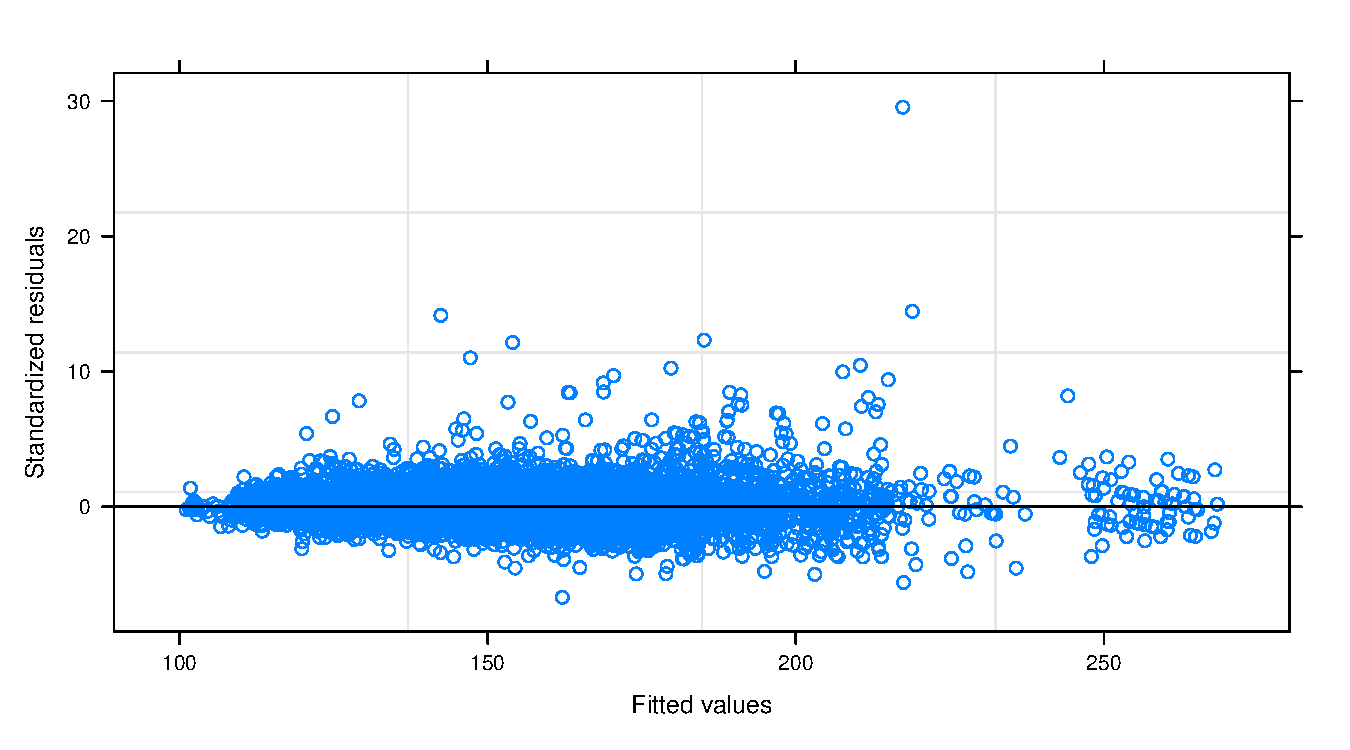
\includegraphics{mixed_model_files/figure-latex/unnamed-chunk-2-1.pdf}

\begin{verbatim}
## Linear mixed-effects model fit by REML
##   Data: EV_data 
##        AIC      BIC    logLik
##   170243.4 170379.8 -85104.69
## 
## Random effects:
##  Formula: ~1 | model
##         (Intercept)
## StdDev:    30.11818
## 
##  Formula: ~1 | vehicle %in% model
##         (Intercept) Residual
## StdDev:    13.98002 9.540513
## 
## Fixed effects:  consumption ~ HDD + CDD + weather_region 
##                                    Value Std.Error    DF  t-value p-value
## (Intercept)                    153.17401  6.899266 21321 22.20149  0.0000
## HDD                              2.49193  0.033174 21321 75.11695  0.0000
## CDD                              3.57815  0.379080 21321  9.43903  0.0000
## weather_regionUpper Hutt         0.46299  1.189344  1238  0.38928  0.6971
## weather_regionChristchurch      -0.92263  1.198540 21321 -0.76979  0.4414
## weather_regionDunedin           13.01269  1.455590  1238  8.93981  0.0000
## weather_regionHamilton           6.02529  1.878845 21321  3.20691  0.0013
## weather_regionNelson            -0.68112  2.089448 21321 -0.32598  0.7444
## weather_regionRotorua            3.39398  1.972163 21321  1.72094  0.0853
## weather_regionClyde              2.70619  2.780982  1238  0.97311  0.3307
## weather_regionPalmerston North  12.31571  2.431945 21321  5.06414  0.0000
## weather_regionStratford          2.23938  3.520545  1238  0.63609  0.5248
## weather_regionNapier             5.27045  3.564989  1238  1.47839  0.1396
## weather_regionInvercargill      12.80979  5.177863  1238  2.47395  0.0135
##  Correlation: 
##                                (Intr) HDD    CDD    wth_UH wthr_rgnCh wthr_D
## HDD                            -0.016                                       
## CDD                            -0.013  0.595                                
## weather_regionUpper Hutt       -0.060 -0.041 -0.013                         
## weather_regionChristchurch     -0.070 -0.067 -0.045  0.395                  
## weather_regionDunedin          -0.046 -0.041 -0.008  0.327  0.324           
## weather_regionHamilton         -0.046 -0.023 -0.017  0.249  0.248      0.199
## weather_regionNelson           -0.033 -0.021 -0.008  0.225  0.234      0.183
## weather_regionRotorua          -0.055 -0.027 -0.015  0.237  0.325      0.195
## weather_regionClyde            -0.031 -0.060 -0.046  0.172  0.170      0.137
## weather_regionPalmerston North -0.034 -0.011  0.000  0.193  0.193      0.156
## weather_regionStratford        -0.034 -0.015 -0.002  0.139  0.132      0.108
## weather_regionNapier           -0.020 -0.010 -0.012  0.131  0.129      0.108
## weather_regionInvercargill     -0.015 -0.017 -0.006  0.095  0.090      0.074
##                                wthr_H wthr_rgnNl wthr_R wthr_rgnCl wth_PN
## HDD                                                                      
## CDD                                                                      
## weather_regionUpper Hutt                                                 
## weather_regionChristchurch                                               
## weather_regionDunedin                                                    
## weather_regionHamilton                                                   
## weather_regionNelson            0.141                                    
## weather_regionRotorua           0.148  0.138                             
## weather_regionClyde             0.106  0.103      0.115                  
## weather_regionPalmerston North  0.376  0.112      0.117  0.082           
## weather_regionStratford         0.077  0.074      0.077  0.053      0.060
## weather_regionNapier            0.084  0.076      0.085  0.060      0.068
## weather_regionInvercargill      0.062  0.050      0.054  0.043      0.045
##                                wthr_S wthr_rgnNp
## HDD                                             
## CDD                                             
## weather_regionUpper Hutt                        
## weather_regionChristchurch                      
## weather_regionDunedin                           
## weather_regionHamilton                          
## weather_regionNelson                            
## weather_regionRotorua                           
## weather_regionClyde                             
## weather_regionPalmerston North                  
## weather_regionStratford                         
## weather_regionNapier            0.043           
## weather_regionInvercargill      0.028  0.030    
## 
## Standardized Within-Group Residuals:
##         Min          Q1         Med          Q3         Max 
## -6.71508814 -0.50911594 -0.04279108  0.43108925 29.62464374 
## 
## Number of Observations: 22592
## Number of Groups: 
##              model vehicle %in% model 
##                 20               1264
\end{verbatim}

\begin{verbatim}
## Linear mixed model fit by REML. t-tests use Satterthwaite's method [
## lmerModLmerTest]
## Formula: consumption ~ HDD + CDD + weather_region + model + (1 | vehicle)
##    Data: EV_data[EV_data$distance != 0, ]
## Weights: 1/distance
## 
## REML criterion at convergence: 194223.9
## 
## Scaled residuals: 
##     Min      1Q  Median      3Q     Max 
## -19.194  -0.315  -0.014   0.271  34.430 
## 
## Random effects:
##  Groups   Name        Variance Std.Dev.
##  vehicle  (Intercept) 233.3402 15.2755 
##  Residual               0.3351  0.5789 
## Number of obs: 22523, groups:  vehicle, 1259
## 
## Fixed effects:
##                                       Estimate Std. Error         df t value
## (Intercept)                          1.302e+02  1.025e+00  1.363e+03 127.027
## HDD                                  2.863e+00  5.022e-02  2.162e+04  57.005
## CDD                                  4.418e+00  5.915e-01  2.163e+04   7.470
## weather_regionUpper Hutt            -8.997e-02  1.366e+00  1.270e+03  -0.066
## weather_regionChristchurch          -2.737e+00  1.379e+00  1.320e+03  -1.984
## weather_regionDunedin                1.085e+01  1.658e+00  1.256e+03   6.540
## weather_regionHamilton               2.451e+00  2.194e+00  1.514e+03   1.117
## weather_regionNelson                -2.623e+00  2.359e+00  1.227e+03  -1.112
## weather_regionRotorua                1.653e+00  2.328e+00  1.742e+03   0.710
## weather_regionClyde                  4.555e-01  3.304e+00  1.431e+03   0.138
## weather_regionPalmerston North       1.546e+01  2.901e+00  2.077e+03   5.329
## weather_regionStratford              1.312e+00  4.039e+00  1.316e+03   0.325
## weather_regionNapier                 4.406e+00  4.014e+00  1.198e+03   1.098
## weather_regionInvercargill           1.322e+01  5.787e+00  1.195e+03   2.284
## modelNissan Leaf (30 kWh)            2.495e+00  1.202e+00  1.401e+03   2.075
## modelNissan Leaf (24 kWh) 2011-2012  1.577e+01  1.367e+00  1.410e+03  11.535
## modelNissan Leaf (40 kWh)            8.722e+00  2.152e+00  1.342e+03   4.052
## modelNissan e-NV200 (24 kWh)         3.452e+01  2.090e+00  1.475e+03  16.515
## modelHyundai Ioniq (EV)             -1.710e+01  3.506e+00  1.314e+03  -4.878
## modelBMW i3                         -1.356e+00  3.587e+00  1.281e+03  -0.378
## modelHyundai Kona (EV)               4.594e+00  4.481e+00  1.221e+03   1.025
## modelRenault Zoe                     1.530e+01  4.287e+00  1.117e+03   3.569
## modelTesla Model 3                   1.367e+01  4.492e+00  1.230e+03   3.042
## modelNissan Leaf (62 kWh)            2.234e+01  4.967e+00  1.400e+03   4.498
## modelKia Niro (EV)                   8.554e+00  5.467e+00  1.183e+03   1.565
## modelTesla Model S                   6.694e+01  7.619e+00  1.353e+03   8.787
## modelVolkswagen e-Golf              -1.956e-01  7.273e+00  1.129e+03  -0.027
## modelTesla Model-X                   1.006e+02  8.306e+00  1.285e+03  12.110
## modelKia Soul                        8.384e+00  9.128e+00  1.080e+03   0.918
## modelMG ZS EV                        1.834e+01  1.093e+01  1.833e+03   1.677
## modelRenault Kangoo (van)            4.114e+01  9.191e+00  1.063e+03   4.476
## modelJaguar I-PACE                   1.119e+02  1.130e+01  1.160e+03   9.900
## modelPeugeot e-208                   6.986e+00  1.640e+01  1.301e+03   0.426
##                                     Pr(>|t|)    
## (Intercept)                          < 2e-16 ***
## HDD                                  < 2e-16 ***
## CDD                                 8.35e-14 ***
## weather_regionUpper Hutt            0.947483    
## weather_regionChristchurch          0.047432 *  
## weather_regionDunedin               8.93e-11 ***
## weather_regionHamilton              0.264022    
## weather_regionNelson                0.266479    
## weather_regionRotorua               0.477855    
## weather_regionClyde                 0.890362    
## weather_regionPalmerston North      1.09e-07 ***
## weather_regionStratford             0.745441    
## weather_regionNapier                0.272569    
## weather_regionInvercargill          0.022527 *  
## modelNissan Leaf (30 kWh)           0.038171 *  
## modelNissan Leaf (24 kWh) 2011-2012  < 2e-16 ***
## modelNissan Leaf (40 kWh)           5.36e-05 ***
## modelNissan e-NV200 (24 kWh)         < 2e-16 ***
## modelHyundai Ioniq (EV)             1.20e-06 ***
## modelBMW i3                         0.705477    
## modelHyundai Kona (EV)              0.305369    
## modelRenault Zoe                    0.000374 ***
## modelTesla Model 3                  0.002397 ** 
## modelNissan Leaf (62 kWh)           7.43e-06 ***
## modelKia Niro (EV)                  0.117951    
## modelTesla Model S                   < 2e-16 ***
## modelVolkswagen e-Golf              0.978553    
## modelTesla Model-X                   < 2e-16 ***
## modelKia Soul                       0.358585    
## modelMG ZS EV                       0.093688 .  
## modelRenault Kangoo (van)           8.42e-06 ***
## modelJaguar I-PACE                   < 2e-16 ***
## modelPeugeot e-208                  0.670201    
## ---
## Signif. codes:  0 '***' 0.001 '**' 0.01 '*' 0.05 '.' 0.1 ' ' 1
\end{verbatim}

\begin{verbatim}
## 
## Correlation matrix not shown by default, as p = 33 > 12.
## Use print(x, correlation=TRUE)  or
##     vcov(x)        if you need it
\end{verbatim}

\begin{verbatim}
## Linear mixed model fit by REML. t-tests use Satterthwaite's method [
## lmerModLmerTest]
## Formula: consumption ~ HDD + CDD + weather_region + (1 | model/vehicle)
##    Data: EV_data[EV_data$distance >= 30, ]
## Weights: 1/distance
## 
## REML criterion at convergence: 186229.3
## 
## Scaled residuals: 
##     Min      1Q  Median      3Q     Max 
## -15.527  -0.358  -0.011   0.323  33.143 
## 
## Random effects:
##  Groups        Name        Variance Std.Dev.
##  vehicle:model (Intercept) 207.9573 14.4207 
##  model         (Intercept) 879.5524 29.6572 
##  Residual                    0.2346  0.4843 
## Number of obs: 22438, groups:  vehicle:model, 1264; model, 20
## 
## Fixed effects:
##                                  Estimate Std. Error         df t value
## (Intercept)                     1.510e+02  6.818e+00  1.844e+01  22.141
## HDD                             3.017e+00  4.350e-02  2.146e+04  69.352
## CDD                             5.696e+00  5.130e-01  2.144e+04  11.102
## weather_regionUpper Hutt       -2.447e-01  1.271e+00  1.255e+03  -0.193
## weather_regionChristchurch     -2.617e+00  1.279e+00  1.316e+03  -2.046
## weather_regionDunedin           1.158e+01  1.547e+00  1.240e+03   7.484
## weather_regionHamilton          4.754e+00  2.058e+00  1.494e+03   2.310
## weather_regionNelson           -2.209e+00  2.201e+00  1.234e+03  -1.004
## weather_regionRotorua           1.853e+00  2.129e+00  1.825e+03   0.871
## weather_regionClyde            -5.344e-02  3.059e+00  1.396e+03  -0.017
## weather_regionPalmerston North  1.211e+01  2.739e+00  1.965e+03   4.421
## weather_regionStratford         1.451e+00  3.751e+00  1.291e+03   0.387
## weather_regionNapier            4.722e+00  3.752e+00  1.178e+03   1.259
## weather_regionInvercargill      1.312e+01  5.409e+00  1.177e+03   2.426
##                                Pr(>|t|)    
## (Intercept)                    9.71e-15 ***
## HDD                             < 2e-16 ***
## CDD                             < 2e-16 ***
## weather_regionUpper Hutt         0.8473    
## weather_regionChristchurch       0.0410 *  
## weather_regionDunedin          1.36e-13 ***
## weather_regionHamilton           0.0210 *  
## weather_regionNelson             0.3157    
## weather_regionRotorua            0.3841    
## weather_regionClyde              0.9861    
## weather_regionPalmerston North 1.04e-05 ***
## weather_regionStratford          0.6989    
## weather_regionNapier             0.2084    
## weather_regionInvercargill       0.0154 *  
## ---
## Signif. codes:  0 '***' 0.001 '**' 0.01 '*' 0.05 '.' 0.1 ' ' 1
\end{verbatim}

\begin{verbatim}
## 
## Correlation matrix not shown by default, as p = 14 > 12.
## Use print(x, correlation=TRUE)  or
##     vcov(x)        if you need it
\end{verbatim}

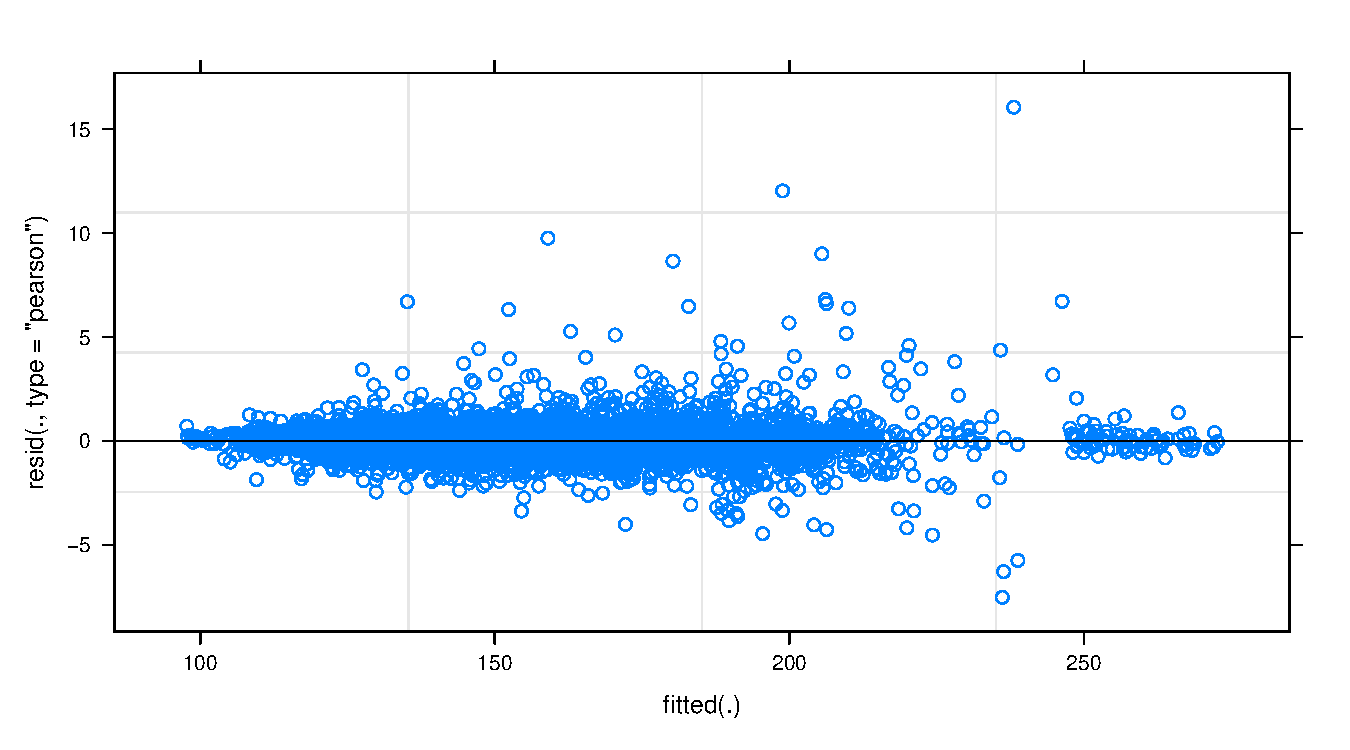
\includegraphics{mixed_model_files/figure-latex/unnamed-chunk-6-1.pdf}

\begin{verbatim}
##                    (Intercept)                            HDD 
##                    153.1740128                      2.4919321 
##                            CDD       weather_regionUpper Hutt 
##                      3.5781487                      0.4629901 
##     weather_regionChristchurch          weather_regionDunedin 
##                     -0.9226282                     13.0126915 
##         weather_regionHamilton           weather_regionNelson 
##                      6.0252890                     -0.6811219 
##          weather_regionRotorua            weather_regionClyde 
##                      3.3939766                      2.7061894 
## weather_regionPalmerston North        weather_regionStratford 
##                     12.3157116                      2.2393805 
##           weather_regionNapier     weather_regionInvercargill 
##                      5.2704466                     12.8097930
\end{verbatim}

\begin{verbatim}
##                                (Intercept)
## Nissan Leaf (24 kWh) 2013-2016  -23.366509
## Nissan Leaf (30 kWh)            -19.451244
## Nissan Leaf (24 kWh) 2011-2012   -7.267122
## Nissan Leaf (40 kWh)            -12.801500
## Nissan e-NV200 (24 kWh)          12.369543
## Hyundai Ioniq (EV)              -37.910707
## BMW i3                          -23.640781
## Hyundai Kona (EV)               -20.522754
## Renault Zoe                     -10.278006
## Tesla Model 3                   -10.628796
## Nissan Leaf (62 kWh)              1.005257
## Kia Niro (EV)                   -12.801947
## Tesla Model S                    39.385149
## Volkswagen e-Golf               -20.929325
## Tesla Model-X                    71.764626
## Kia Soul                        -11.960587
## MG ZS EV                          2.377236
## Renault Kangoo (van)             32.427778
## Jaguar I-PACE                    63.278363
## Peugeot e-208                   -11.048674
\end{verbatim}

\begin{verbatim}
## NULL
\end{verbatim}

\end{document}
